% nroy-images.tex
% Study note: general procedure + planted village PoC with figures.
% Compile:  xelatex nroy-images.tex
% Not a specification. METHODOLOGY.md wins if they disagree.
\documentclass[11pt]{article}

\usepackage[letterpaper,margin=22mm]{geometry}
\usepackage{fontspec}
\setmainfont{Menlo}[
  Scale=0.86,
  Ligatures=TeX,
  BoldFont={Menlo Bold},
]
\usepackage{amsmath,amssymb,amsthm}
\usepackage{booktabs}
\usepackage{array}
\usepackage{tabularx}
\usepackage{enumitem}
\usepackage{graphicx}
\usepackage{microtype}
\usepackage{setspace}
\usepackage{titlesec}
\usepackage{tikz}
\usetikzlibrary{arrows.meta,positioning,fit,calc,chains}
\usepackage{capt-of}
\usepackage{xcolor}
\usepackage[hidelinks]{hyperref}

\definecolor{ink}{HTML}{111111}
\definecolor{rule}{HTML}{222222}
\definecolor{wash}{HTML}{F4F4F4}
\definecolor{line}{HTML}{555555}

\setstretch{1.12}
\pagestyle{plain}
\setlength{\parindent}{0pt}
\setlength{\parskip}{0.55em}
\setlist[itemize]{leftmargin=1.4em,itemsep=0.15em,topsep=0.25em}
\setlist[enumerate]{leftmargin=1.6em,itemsep=0.15em,topsep=0.25em}

\titleformat{\section}[block]
  {\normalsize\bfseries\color{ink}}
  {\thesection}{0.7em}{}
  [\vspace{-0.4em}{\color{rule}\titlerule[0.4pt]}]
\titleformat{\subsection}[runin]
  {\normalsize\bfseries\color{ink}}
  {\thesubsection}{0.6em}{}[.~]
\titlespacing*{\section}{0pt}{1.4em}{0.7em}
\titlespacing*{\subsection}{0pt}{0.9em}{0.4em}

\newcommand{\NROY}{\mathrm{NROY}}
\newcommand{\hm}{\mathrm{hm}}
\newcommand{\cv}{\mathrm{cv}}
\newcommand{\expset}{\mathrm{exp}}
\newcommand{\thr}{\tau_{\mathrm{I}}}
\newcommand{\prem}{\psi}
\newcommand{\interior}{\operatorname{int}}
\newcommand{\Iols}{I_{\mathrm{OLS}}}
\newcommand{\Ie}{I_{E2}}

\begin{document}

{\centering
{\large\bfseries Not-ruled-out images of policy contrasts}\\[0.35em]
{\small A general procedure, with a planted village ABM as illustration}\\[0.45em]
{\small ECN 593 study note \textperiodcentered\ freeze 2026-08-26 / AMENDMENT-02
\textperiodcentered\ PoC figures 2026-08-28 / note updated 2026-10-05}\\[0.8em]
}

\noindent
This note writes the pipeline in generality first, then uses one
implemented simulator as an example. The reporting object is a
\emph{not-ruled-out image} of a named policy contrast. That is the same
\emph{reporting logic} as a partially identified set---do not replace a
set by a convenient point---not a claim that the object has the
theorems of a Manski identified set.

Lectures in \texttt{docs/lectures/} were drafted \emph{before} waves.
They are not this write-up. Numbers below come from the planted JSON
in \texttt{results/} and the archived F-empty file. Foil~1 on this pin
is OLS-HC1, not a forest and not BCF. Overlay verdicts are written as
set relations on subsets of \(\mathbb{R}\) (Section~\ref{sec:geometry}).

%----------------------------------------------------------------
\section{The planner's problem}

A planner compares assignment rules (policies) that act on a population
of interfering units. Individual contrasts $Y_i(1)-Y_i(0)$ are not the
target: under interference the argument of $Y_i$ is the whole assignment
vector. The natural estimand is a contrast of rules,
\begin{equation}
  \theta(\pi,\pi';c)
  \;=\;
  \mathbb{E}_c\!\left[\bar Y(\pi)\right]
  \;-\;
  \mathbb{E}_c\!\left[\bar Y(\pi')\right],
\end{equation}
where $c$ indexes a complete data-generating process (a kernel, an ABM,
a structural model) and the expectation is over whatever residual
randomness the kernel still has once $c$ is fixed.

The planner does not know $c$. What she has is a class of kernels
$\{f(\,\cdot\,;c):c\in C\}$ and a low-dimensional vector of moments $z$
that she is willing to treat as the right functionals of the system.
(``Willing'' here is an identifying assumption about \emph{which
summaries to match}. It is not who named $\theta$. Augusto froze
$\theta_2$ as a contrast of terminal means in METHODOLOGY.md §4.)
History matching then \emph{rules out} calibrations. It does not
produce a posterior over worlds. The decision-relevant object is not
the surviving set in parameter space. It is the image of $\theta$ over
that set.

Two further incompletenesses sit beside calibration, and must not be
folded into the same interval: (i)~the scoring of the outcome $Y$
(which operationalization?), and (ii)~the fact that default estimators
are one-world objects. The procedure below keeps the three sources on
separate axes.

%----------------------------------------------------------------
\section{Objects}

\paragraph{Kernel.}
A complete mapping $f$ from $(c,\omega,\pi)$ to a panel
$(Y_T,D,X,A)$. Here $\omega$ is simulation noise, $\pi$ is an
assignment rule, $A$ is a (possibly stochastic) network, $X$ are
covariates. The kernel is complete: incompleteness lives in $c$, not in
unobserved counterfactuals inside $f$ (Section~\ref{sec:po}).
Implemented as vectorized algebra (\texttt{kernel.py}), not as a
turtle-by-turtle framework. NetLogo would be a twin of the same $f$,
not a different science.

\paragraph{Box.}
$C\subset\mathbb{R}^d$ is the a priori range of free coordinates of
$c$. Coordinates that are not up for calibration (in the example,
$\eta$) are frozen inside $f$, not inside $C$.

\paragraph{Named estimands.}
A short list of contrasts, declared before any wave. Under interference
the argument of $Y_i$ is the whole assignment, so
\begin{equation}
  \theta(\pi,\pi';c)
  \;=\;
  \mathbb{E}_c\!\left[\bar Y_T(\pi)\right]
  \;-\;
  \mathbb{E}_c\!\left[\bar Y_T(\pi')\right].
\end{equation}
In the illustration the named list is
\begin{align}
  \theta_1(c)
  &= \mathbb{E}_c[\bar Y_T\mid\pi_1]-\mathbb{E}_c[\bar Y_T\mid\pi_0],
  \\
  \theta_2(c)
  &= \mathbb{E}_c[\bar Y_T\mid\pi_2]-\mathbb{E}_c[\bar Y_T\mid\pi_0]
  \quad\text{(headline)},
  \\
  \prem(c)
  &= \theta_2(c)-\theta_1(c)
  \quad\text{(targeting premium)}.
\end{align}
$\delta_{\mathrm{spill}}(c)$ is a separate exposure-mapped spillover on
the only arm that has a design (Section~\ref{sec:design}). Notation:
the history-matching threshold is $\thr$, not $\prem$. The two must not
share a glyph. Expectations are over $\omega$ only ($\pi_0$ and $\pi_2$
are deterministic given $A$; $\pi_1$'s extra randomness is part of
$\omega$).

$\theta$ is defined on the \emph{terminal} village mean $\bar Y_T$, not
on the 20-day path. That is how the functional was named, not a proof
that path summaries would be wrong. A path functional would be a
different freeze, and then $M$ and $z$ should be path summaries too.

\paragraph{Moment map.}
$M:C\to\mathbb{R}^k$ with $k<d$ by design. Underidentification in $c$
is intended; the deliverable is a set in $c$-space. Whether $\theta$
moves on that set is empirical. $M$ is not a menu of outcome scorings.

\paragraph{Anchors.}
$z\in\mathbb{R}^k$ is the target for $M$. In a simulation study $z$ may
be planted from a known $c^\star\in C$. In an empirical study $z$ is
external. Either way, $z$ is frozen before waves.

\paragraph{Implausibility.}
\begin{equation}
  I(c)
  \;=\;
  \bigl(z-\widehat M(c)\bigr)^{\!\top}
  V(c)^{-1}
  \bigl(z-\widehat M(c)\bigr),
\end{equation}
a squared Mahalanobis discrepancy, not a distance.
$V(c)=\mathrm{diag}\bigl(\sigma^2_{\mathrm{samp}}(z)
+\sigma^2_{\mathrm{MC}}(\widehat M(c))
+\delta^{\circ 2}\bigr)$.
The three pieces are sampling error in $z$, Monte Carlo error in the
candidate moment, and an explicit model-discrepancy budget $\delta$.
$V$ does not contain survey-measure noise.

\paragraph{Not-ruled-out-yet set.}
$\NROY=\{c\in C:I(c)\le\thr\}$. Membership means we are not entitled to
discard $c$. It does not mean $c$ is observationally equivalent to the
truth, and it is not a posterior.

\paragraph{Images.}
\begin{align}
  \Theta_{\hm}
  &= \{\theta_2(c):c\in\NROY\},
  &
  \Theta_{\expset}
  &= \{\delta_{\mathrm{spill}}(c):c\in\NROY\}.
\end{align}
Reported as empirical $[L,U]$ over a pre-registered sample of
survivors. No measure (uniform, posterior, \ldots) is placed on
$\NROY$. Width is empirical: distinct survivors \emph{can} map to
different $\theta$; they need not.

\paragraph{Diagnostic worlds.}
Two points $c_0^{\min I}$, $c_0^{\mathrm{med}\,I}$, functions of $I$
only. Never of $\theta$. ``Best match'' and ``non-extremal'' are the
rationales; neither is theoretically privileged.

\paragraph{Measures.}
Scorings $m$ of $Y_T$, frozen as a menu, admitted or excluded by a
pre-declared restriction. $M^\star$ is a set of measures, not a subset
of $\NROY$. $\Theta_{\cv}(c_0)$ is the image of the estimand over
$M^\star$ at that world.

\paragraph{Panel.}
One run of $f$ is one micro-dataset
\begin{equation}
  \mathcal{D}(c,\omega,\pi)
  \;=\;
  \bigl\{(Y_{iT},\,D_i,\,X_i,\,A_{i\cdot})\bigr\}_{i=1}^{N}.
\end{equation}
World $\neq$ panel. One-world means the estimator is not given
$\NROY$; it conditions on one $c$. One panel is one $\omega$. Kernel
truth $\theta(c)$ is still one-world and uses $R=200$ paired reps.
Averaging a foil over 200 panels at the same $c_0$ would still be
one-world.

\paragraph{Foils.}
One-world estimators fitted at each $c_0$ on \emph{one} panel. Each
foil is judged against \emph{its own} image and against truth at that
world (Section~\ref{sec:geometry}). They are not candidates for
$\Theta_{\hm}$.

%----------------------------------------------------------------
\section{Potential outcomes, and what counts as data}
\label{sec:po}

Hahn / Rubin--Neyman with SUTVA: $Y_i=Y_i(D_i)$, $D_i\in\{0,1\}$. One
of two numbers per person is missing. That missingness \emph{is} the
incompleteness. BCF, an honest forest, or OLS-HC1 is a gold-standard
interval for that SUTVA functional, given one dataset, at one world.
The ruler, not the villain. Not ``the forest failed under
interference.''

This class drops SUTVA ($\gamma>0$, peer \emph{outcomes}):
$Y_i=Y_i(\mathbf{d})$, $\mathbf{d}\in\{0,1\}^N$. The individual
contrast $Y_i(1)-Y_i(0)$ is undefined unless everyone else's assignment
is named. The well-defined object is a Hudgens--Halloran overall /
policy contrast $\theta(\pi,\pi';c)$ as above.

In the \emph{field}, other $\bar Y(\pi)$ are still missing (one
campaign). That would be Manski incompleteness in the potential
outcomes. In the \emph{simulator}, $f$ is complete: run both arms, pair
$\omega$, subtract. Nothing inside $f$ is an unobserved counterfactual.
Remaining incompleteness is which $c\in C$ (five free knobs, three
moments). $\Theta_{\hm}=\{\theta_2(c):I(c)\le\thr\}$ is a
not-ruled-out image, not a Manski identified set and not a set of
still-possible $Y_i(0)$. Same \emph{reporting logic} (do not replace a
set by a convenient point); not the same theorem.

$d>k$ underidentifies $c$. Width of $\Theta_{\hm}$ is measured. Matching
arm \emph{levels} while $\theta_2$ is a \emph{contrast against control}
makes unpinning possible, not a theorem (Section~\ref{sec:zcontrol}).

\paragraph{Only two objects have empirical analogs.}
\begin{center}
\small
\begin{tabular}{@{}llp{55mm}@{}}
\toprule
empirical analog & simulator object & who consumes it \\
\midrule
one campaign's micro data
  & one panel $\mathcal{D}(c,\omega,\pi)$
  & OLS-HC1, H\'ajek \\
calibration targets
  & $z$ (plus sampling variances, $\delta$)
  & $I(c)$, $\NROY$ \\
survey operationalization
  & $s=m(Y_T)$
  & foils / $\Theta_{\cv}$ \\
\bottomrule
\end{tabular}
\end{center}
Not data: LHS points, moment and estimand Monte Carlo reps, $\NROY$
survivors, the image sample, $\theta(c)$. Those are probes of $f$.
$\NROY$ points are arguments of $\theta(\cdot)$, not extra surveys.

%----------------------------------------------------------------
\section{Order of operations}

The order is part of the identification statement. Using $\theta$ to
decide which $c$ survive is fishing.

\begin{enumerate}
  \item Freeze $f$, $C$, $z$, $\delta$, $\thr$, the estimands, the
        measure menu and its admission rule, and the $c_0$ rule.
  \item Draw the environment $(A,X)$ once.
  \item History-match: evaluate $I(c)$ on a space-filling design,
        keep $I\le\thr$, optionally concentrate later waves on the
        surviving box. $\NROY$ is the union of survivors.
        Empty $\NROY$ is a finding: the pair $(f,z)$ is rejected.
        Do not move $\thr$ or $\delta$ after seeing the waves.
  \item Leg~A. Sample survivors. Compute $\theta(c)$ and
        $\delta_{\mathrm{spill}}(c)$ from the kernel. Report
        $\Theta_{\hm}$ and $\Theta_{\expset}$ as $[L,U]$.
  \item Leg~B. At each $c_0$, fit the one-world foils on a single
        panel. Compare each interval to its own image and to kernel
        truth at that $c_0$.
  \item Measures. At those same $c_0$, score $Y$ under each $m$,
        admit, report $\Theta_{\cv}$. Side branch, not a gate on
        legs A and B.
\end{enumerate}

\vspace{0.6em}
\begin{center}
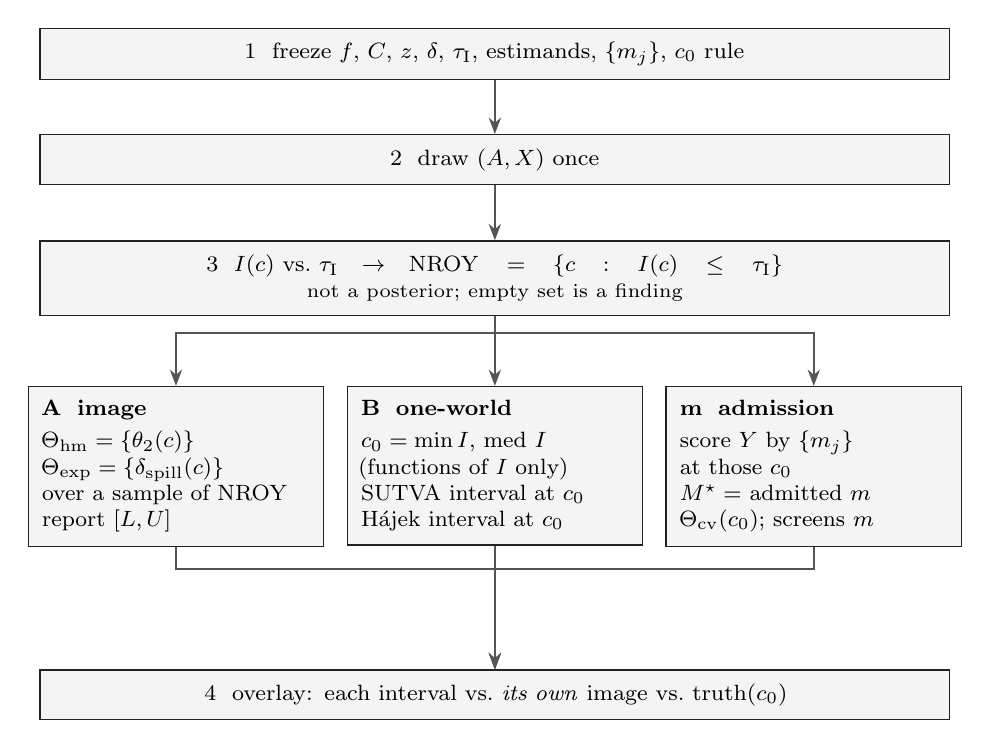
\begin{tikzpicture}[
  font=\footnotesize,
  >=Stealth,
  box/.style={
    draw=rule, line width=0.45pt, fill=wash,
    inner sep=5pt, align=left, anchor=north,
  },
  wide/.style={box, text width=112mm, align=center},
  col/.style={box, text width=34mm},
  arr/.style={->, line width=0.65pt, color=line},
]
  \node[wide] (freeze) at (0,0)
    {1~~freeze $f$, $C$, $z$, $\delta$, $\thr$, estimands, $\{m_j\}$, $c_0$ rule};
  \node[wide] (env) at (0,-1.35)
    {2~~draw $(A,X)$ once};
  \node[wide] (hm) at (0,-2.70)
    {3~~$I(c)$ vs.\ $\thr$ ~~$\to$~~ $\NROY=\{c:I(c)\le\thr\}$\\
     {\scriptsize not a posterior; empty set is a finding}};

  \node[col] (A) at (-4.05,-4.55)
    {\textbf{A~~image}\\[0.25em]
     $\Theta_{\hm}=\{\theta_2(c)\}$\\
     $\Theta_{\expset}=\{\delta_{\mathrm{spill}}(c)\}$\\
     over a sample of $\NROY$\\
     report $[L,U]$};
  \node[col] (B) at (0,-4.55)
    {\textbf{B~~one-world}\\[0.25em]
     $c_0=\min I$, med $I$\\
     (functions of $I$ only)\\
     SUTVA interval at $c_0$\\
     H\'ajek interval at $c_0$};
  \node[col] (M) at (4.05,-4.55)
    {\textbf{m~~admission}\\[0.25em]
     score $Y$ by $\{m_j\}$\\
     at those $c_0$\\
     $M^\star=$ admitted $m$\\
     $\Theta_{\cv}(c_0)$; screens $m$};

  \node[wide] (ov) at (0,-8.15)
    {4~~overlay: each interval vs.\ \emph{its own} image vs.\ truth$(c_0)$};

  \draw[arr] (freeze.south) -- (env.north);
  \draw[arr] (env.south) -- (hm.north);
  \draw[arr] (hm.south) -- ++(0,-0.22) -| (A.north);
  \draw[arr] (hm.south) -- (B.north);
  \draw[arr] (hm.south) -- ++(0,-0.22) -| (M.north);
  \draw[arr] (A.south) -- ++(0,-0.28) -| (ov.north);
  \draw[arr] (B.south) -- (ov.north);
  \draw[arr] (M.south) -- ++(0,-0.28) -| (ov.north);
\end{tikzpicture}
\end{center}
\captionof{figure}{Order of operations. Legs A and B, and the measurement
branch, are three reports. They do not merge into a single
``construct-identified-robust'' object.}
\label{fig:pipe}

%----------------------------------------------------------------
\section{Design of exogenous quantities}

Everything below is frozen before waves. The justifications are
design justifications, not data-dependent ones.

\subsection{Threshold $\thr$}
$I(c)$ is a $k$-dimensional squared Gaussian form if $z-\widehat M$
were normal with covariance $V$. Taking $\thr=F^{-1}_{\chi^2_k}(0.95)$
is the conventional history-matching cutoff (a 95\,\% ellipsoid). It is
a ruling-out convention, not a posterior credible region. Moving
$\thr$ after seeing $\NROY$ would convert a pre-registered filter into
a fit.

\subsection{Discrepancy $\delta$}
Kennedy--O'Hagan discrepancy is the admission that even the right $c$
need not hit $z$ exactly, because $f$ is not the world. On a correctly
specified simulator $\delta$ is conservative: $\NROY$ is larger than a
$\delta=0$ match. Keeping a pre-declared $\delta$ anyway separates
``the analyst's budget'' from ``what the DGP can hit.'' Loosening
$\delta$ after a wave is the same sin as loosening $\thr$.

\subsection{The box $C$}
Wide enough that underidentification is possible ($d>k$), narrow enough
that every coordinate is economically signed (persistence, peer
weight, and own-treatment shift positive; intercept not so free that
$Y$ saturates for every $c$). Excluding $\gamma=0$ is a statement of
subject-matter: the paper is about interference; a no-interference
world surviving calibration would be its own finding and must not be
slipped in.

\subsection{How $c$ is drawn}
Nobody picks a favourite five-tuple by looking at $\theta$. Wave~1 is a
Latin Hypercube of 1000 points in $C$. Each candidate is kept iff
$I(c)\le\thr$. Waves 2--3 redraw LHS in the survivors' bounding box,
inflated 20\,\% and clipped back to $C$. $\NROY$ is the \emph{union}
across waves. The plant $c^\star$ is the centre of $C$, chosen without
looking at $\theta$. Diagnostic $c_0$ are min $I$ and median $I$ on
that union.

\subsection{Anchors $z$}
\label{sec:zcontrol}
Two admissible sources, with different claims.

\emph{External $z$.} Moments with a policy story and a kernel analog.
If no $c\in C$ satisfies $I(c)\le\thr$, that is F-empty: the pair
$(f,z)$ is rejected. That finding is about the analog, not about
$\theta$. Empty is the opposite of a wide $\Theta$.

\emph{Planted $z$.} $z:=\widehat M(c^\star)$ at a $c^\star$ chosen
without looking at $\theta$. The illustration uses the centre of $C$.
Planting makes $\NROY$ feasible by construction and makes
$\theta_{\mathrm{true}}$ known, which is the only place an overlay is
checkable.

There are \emph{three} moments, not five. Five is $d$, the free
coordinates of $C$ ($\alpha,\beta,\gamma,\kappa,\sigma_\varepsilon$).
$\eta$ is frozen inside $f$, not a moment and not in $C$. The three
slots, in order:
\begin{center}
\small
\begin{tabular}{@{}lll@{}}
\toprule
slot (historical name) & village functional & arm \\
\midrule
\texttt{level\_imm} & $\mathbb{E}[\bar Y_T\mid\pi_2]$ & hub level \\
\texttt{gradient\_edu} & $\mathrm{corr}(Y_T,x_1\mid\pi_2)$ & literacy gradient \\
\texttt{level\_internet} & $\mathbb{E}[\bar Y_T\mid\pi_1]$ & random level \\
\bottomrule
\end{tabular}
\end{center}
Control's mean $\mathbb{E}[\bar Y_T\mid\pi_0]$ is \emph{not} in $z$.
That is how $z$ was named, not a theorem that it must be omitted.
World Bank slots were three campaign-era / country aggregates
(immunization, education gradient, internet); there is no untreated
planet in that file. After F-empty, AMENDMENT-02 kept the same three
functionals and planted them at $c^\star$. METHODOLOGY does not contain
a paragraph ``exclude $\pi_0$ so that $\theta_2$ is set-identified.''
Underidentification of $c$ is designed ($d=5$, $k=3$). Unpinning of
$\theta_2$ is a \emph{possible} consequence of matching levels while
$\theta_2$ is a contrast against an unmatched control, plus $\delta$.
Width remains measured.

If control were added, $k=4$ and $c$ would still be a set, but
$\theta_2$ would sit close to a difference of two matched moments plus
the $\delta$ slop. That would be a different freeze. Neither adding it
to manufacture tightness nor dropping it to manufacture width is a
scientific reason.

The illustration ran both sources. Country aggregates as $z$ returned
F-empty and were archived. The overlay uses the plant.

\subsection{Diagnostic $c_0$}
Min $I$ mimics best-fit / MSM practice. Median $I$ is a non-extremal
rule on the same ranking. Both are functions of moment fit, not of the
estimand. Two worlds, not four hundred: looping the estimator over
every survivor answers ``what if we gave the learner the calibration
set,'' which default practice does not.

\subsection{Foils}
\label{sec:design}
Foil~1 is a SUTVA one-world interval at $c_0$. The frozen role is that
ruler: an honest interval \emph{conditional on a world}, not a
defendant charged with failing under interference. Preferred software
is an honest causal forest; this pin does not load it
(\texttt{econml} against \texttt{numpy==2.4.6}). The run therefore uses
the declared fallback: OLS of the scored outcome on $D$ given $X$, HC1
interval. Report the name. Do not call it BCF. BCF remains an extra
row only if asked for, same $c_0$, no new rule.

On one $\pi_2$ panel the regression is
$s_i=\alpha+\tau D_i+X_i^\top\eta+u_i$. Stack
$Z_i=(1,\,D_i,\,X_i')\in\mathbb{R}^{k}$ with $k=5$ here
(intercept, $D$, three covariates). OLS
$\hat\beta=(Z^\top Z)^{-1}Z^\top s$, and $\hat\tau$ is the $D$
coordinate. HC1 is the degrees-of-freedom sandwich
\begin{equation}
  \widehat{\mathrm{Var}}_{\mathrm{HC1}}(\hat\beta)
  \;=\;
  \frac{n}{n-k}
  \,(Z^\top Z)^{-1}
  \Bigl(\sum_{i=1}^{n}\hat u_i^2\,Z_i Z_i^\top\Bigr)
  \,(Z^\top Z)^{-1}.
\end{equation}
$\Iols$ is $\hat\tau\pm z_{1-\alpha/2}\,\mathrm{SE}(\hat\tau)$ with
$\mathrm{SE}$ the square root of the $D$ diagonal. At $N=800$,
$n/(n-k)=800/795\approx 1.006$; the name is the convention, not a
material correction. Rows are treated as uncorrelated. That is already
a SUTVA-style assumption, not a network standard error. On the hub
panel $D$ \emph{is} ``being a hub,'' so $\hat\tau$ lives near
$\delta_{\mathrm{dir}}$ (hubs vs non-hubs inside one campaign), not
near $\theta_2$.

Foil~2 is design-based and exposure-mapped, and therefore lives only on
an arm with a known assignment \emph{lottery}. ``Design'' here is not
``research design'' and not ``we designed an ABM.'' It means: can one
write $p_i=\Pr_\pi(D_i=1)$ and exposure probabilities from a known hat,
before seeing $Y$?

$\pi_1$ is SRSWOR: simple random sample without replacement. Seed
exactly 80 of 800 households; every 80-subset equally likely; no
repeats. Inclusion $p_i=80/800=1/10$. Neighbour counts among the
untreated are hypergeometric, which is how $p_{i,S}$ are written
without touching $(\alpha,\beta,\gamma)$. $\pi_2$ (top-80 degree) has
no hat: given $A$, $p_i\in\{0,1\}$. Inverse-probability weights are
undefined. That un-reachability is reported, not walked around.

``Estimable from one designed panel'' means: from one realized
randomized campaign plus the known lottery, form
$\widehat\delta_{\mathrm{spill}}$ and $\widehat\delta_{\mathrm{dir}}$.
It does \emph{not} mean $\theta_2$ is identified from one campaign.
$\theta_2$ needs $\pi_2$ and $\pi_0$. Even a field hub-campaign does
not see control, and was not a lottery.

Exposure $g_i=(D_i,s_i)$ with the same $k_i$ as in the kernel
(degree, isolates patched):
\begin{equation}
  k_i=\max\Bigl(\sum_j A_{ij},\,1\Bigr),\qquad
  s_i=\frac{\sum_{j:A_{ij}=1}D_j}{k_i}.
\end{equation}
$s_i$ is the share of neighbours' \emph{treatment}, not neighbours'
outcomes. Isolates have $k_i=1$ and $s_i=0$. Path $A{-}B{-}C{-}D$,
treat $\{B\}$: $s=(1,\,0,\,0.5,\,0)$. Strata at cut $0.25$ are the
sets
\begin{align*}
  S_1  &= \{i:D_i=1\}, \\
  S_{0a} &= \{i:D_i=0,\; s_i=0\}, \\
  S_{0b} &= \{i:D_i=0,\; 0<s_i<0.25\}, \\
  S_{0c} &= \{i:D_i=0,\; s_i\ge 0.25\}.
\end{align*}
On that path: $A,C\in S_{0c}$, $B\in S_1$, $D\in S_{0a}$, $S_{0b}=\emptyset$.
If any cell has fewer than 20 agents in a replication, $S_{0b}$ is
merged into $S_{0c}$ for all reps of that world.

Kernel truth uses unweighted cell means of oracle $Y$, then averages
over random-arm reps:
\begin{equation}
  \delta_{\mathrm{dir}}(c)=\mu_{S_1}-\mu_{S_{0a}},\qquad
  \delta_{\mathrm{spill}}(c)=\mu_{S_{0c}}-\mu_{S_{0a}}.
\end{equation}
Foil~2 replaces $\mu_S$ by the H\'ajek mean on one $\pi_1$ panel,
\begin{equation}
  \widehat\mu_S
  \;=\;
  \frac{\sum_i \mathbf{1}\{i\in S\}\,Y_i/p_{i,S}}
       {\sum_i \mathbf{1}\{i\in S\}/p_{i,S}}.
\end{equation}
Glue the two $\mu_S$ and the oracle gate is unreadable. The exposure
map is neighbour-$D$; the kernel peer term is neighbour-$Y$ over $T$
ticks (a S\"avje-style misspecification of the map). That is a
limitation of Foil~2, not a license to replace it with a second SUTVA
learner.

Foil~2 does \emph{not} estimate $\theta_2$. Two different one-world
referents, neither of which is the calibrated-simulator report: Hahn
classroom $\to$ Foil~1; a network RCT that admits interference and uses
an exposure map (Aronow--Samii family) $\to$ Foil~2. The goal of the
second row is an interference-aware interval that (i)~can write
spillover, (ii)~is identified by a lottery from one panel, (iii)~still
does not consume $\NROY$, so $\Ie$ versus $\Theta_{\expset}$ isolates
calibration after architecture (Section~\ref{sec:geometry}). Rank
replacements by that goal. Dropping Foil~2, or swapping it for BCF,
returns the architecture/calibration confound. Stochasticizing
hub-seeding so IPW can hit it is a different policy.
$\Theta_{\expset}$ is the image of the \emph{kernel}
$\delta_{\mathrm{spill}}(c)$, not of the H\'ajek interval.

\subsection{Measures}
A short menu, including a positive control (oracle $s=Y$) and a scoring
designed to fail a restriction stated in English before the wave
(``must not load on a treatment-channel covariate''). Admission is
mechanical. It does not look at $\theta$.

\subsection{Monte Carlo budgets}
Moment evaluations use fewer replications than estimand evaluations:
ruling-out has to be cheap enough to search $C$; $\theta(c)$ is
computed only on survivors. The plant uses the estimand budget so that
$z$ is not noisier than the object we will later quote.

%----------------------------------------------------------------
\section{Interval geometry}
\label{sec:geometry}

Sampling intervals and images are subsets of $\mathbb{R}$. Verdicts
are inclusions, not slogans.

Let $I=[\iota_L,\iota_U]\subset\mathbb{R}$ be a closed sampling
interval (a foil CI at one $c_0$) and let $\Theta=[L,U]\subset\mathbb{R}$
be the reported image of the \emph{same} functional over a
pre-registered sample of $\NROY$ (empirical min/max; not a continuum
and not a posterior). Write $\interior(\Theta)=(L,U)$.

Implemented labels (METHODOLOGY §10; \texttt{classify\_interval}):
\begin{align}
  \text{F-HONEST}
  &\iff \Theta\subseteq I, \\
  \text{F-OVERCONF}
  &\iff I\subset\interior(\Theta).
\end{align}
Anything else is unnamed --- no third finding after the freeze ---
including
\begin{equation}
  I\cap\Theta=\emptyset
  \qquad\text{and}\qquad
  I\cap\Theta\neq\emptyset
  \text{ with neither inclusion}.
\end{equation}
The code does not additionally test whether $\theta_{\mathrm{true}}$
sits outside $I$. METHODOLOGY's prose ``and excludes $\theta_{\mathrm{true}}$
or parts of $[L,U]$'' is already implied by $I\subset\interior(\Theta)$
for the image endpoints; $\theta_{\mathrm{true}}(c_0)$ is checked
separately by the oracle gate.

Oracle gate (harness, not a finding):
\begin{equation}
  \theta_{\mathrm{true}}(c_0)\in I
  \quad\text{or, for Foil~2,}\quad
  \delta_{\mathrm{spill}}(c_0)\in\Ie.
\end{equation}
The point estimate is unused. Fail $\Rightarrow$ stop; do not read
overlay stickers.

Each foil versus \emph{its own} image:
\begin{equation}
  (\Iols,\;\Theta_{\hm}),
  \qquad
  (\Ie,\;\Theta_{\expset}).
\end{equation}
Cross-functional geometry ($\Iols$ against $\Theta_{\hm}$ when OLS is
not $\theta_2$) is reported as a set relation, not forced into F-*.

Two gaps must not be dumped into one interval. Write
\begin{align*}
  \mathcal{A}
  &= \text{architecture (SUTVA vs exposure map vs kernel)}, \\
  \mathcal{C}
  &= \text{calibration (which }c\in\NROY\text{)}.
\end{align*}
$\Iols$ versus $\Theta_{\hm}$ can mix $\mathcal{A}$ and $\mathcal{C}$
when the functionals differ. Foil~2 is the attempt to handle
$\mathcal{A}$ first: it can write spillover and still does not see
$\NROY$. Then, in order,
\begin{enumerate}
  \item $\delta_{\mathrm{spill}}(c_0)\in\Ie$
        --- architecture and sampling OK \emph{at the world};
  \item $\Ie\subset\interior(\Theta_{\expset})$
        --- residual width is variation of the \emph{same} functional
        across surviving $c$.
\end{enumerate}
That pair is what ``$\Ie$ versus $\Theta_{\expset}$ isolates
calibration after architecture'' means. The leftover set
$\Theta_{\expset}\setminus\Ie$ is not a sampling CI and is not a
SUTVA misspecification residual. F-OVERCONF-E2 is only the sticker
for (2). It is almost automatic once (1) holds and
the length of $\Theta_{\expset}$ exceeds sampling noise. Empty or covering images
are also allowed findings; the interesting object is the width, not
the label.

%----------------------------------------------------------------
\section{Illustration: a planted village}

One large village, $N=800$ households, acquaintance network
$G(N,4/N)$ (mean degree $\approx 4$). $Y_{i,t}\in(0,1)$ is
preventive-practice intensity---a score, not a country coverage rate.
Covariates: literacy $x_1$, resources $x_2$, baseline propensity $x_3$.
Three rules seed 80 households from $t=0$: none ($\pi_0$); SRSWOR
($\pi_1$, the only arm with a design); the 80 highest-degree
households ($\pi_2$, deterministic given $A$).

The kernel is linear-in-means with logistic saturation. For
$t=0,\ldots,T-1$ with $T=20$,
\begin{equation}
  Y_i(t+1)
  \;=\;
  \Lambda\!\Bigl(
    \alpha + \beta Y_i(t)
    + \gamma \frac{\sum_{j\in N(i)} Y_j(t)}{k_i}
    + \eta\cdot X_i
    + \kappa D_i
    + \varepsilon_i(t)
  \Bigr),
\end{equation}
$\Lambda(z)=1/(1+e^{-z})$, $\varepsilon_i(t)\sim N(0,\sigma_\varepsilon^2)$.
Peers enter as neighbours' \emph{lagged practice}, not as neighbour
treatment. The five free coordinates and the frozen $\eta$ are
\begin{center}
\small
\begin{tabular}{@{}llp{72mm}@{}}
\toprule
 & box / value & role \\
\midrule
$\alpha$ & $[-2.5,-0.5]$ & intercept of the index \\
$\beta$ & $[0.05,0.60]$ & own-lag persistence \\
$\gamma$ & $[0.05,0.80]$ & peer weight; $0$ excluded \\
$\kappa$ & $[0.25,2.50]$ & own-treatment shift (same $\kappa$ on every arm) \\
$\sigma_\varepsilon$ & $[0.01,0.40]$ & sd of $\varepsilon$, not a standard error \\
$\eta$ & $(0.05,0.10,0.02)$ & literacy, resources, propensity; not calibrated \\
\bottomrule
\end{tabular}
\end{center}

$c^\star$ is the centre of $C$:
$(-1.5,\,0.325,\,0.425,\,1.375,\,0.205)$.
Frozen $z=\widehat M(c^\star)=(0.264,\,0.050,\,0.262)$ --- hub-arm
mean $Y_T$, corr$(Y_T,x_1)$ on the hub arm, random-arm mean $Y_T$.
The control mean is \emph{not} in $z$, so $\theta_2$ (a contrast
against control) is not a moment being matched.
$\delta=(0.02,0.05,0.02)$ and
$\thr=F^{-1}_{\chi^2_3}(0.95)\approx 7.81$ are the same numbers used in
the rejected country-total attempt.

The graph $A$ is drawn once and not calibrated. Connectivity is not the
latent being measured. The measurement layer scores $Y$, not edges.

%----------------------------------------------------------------
\section{PoC results}

\subsection{External $z$ failed}
Matching the same kernel to rescaled World Bank country totals
(DPT coverage, education--immunization correlation, internet users;
fetched 2026-08-12) ruled out every $c$. Wave~1 kept 0 of 1000.
Minimum $I=204$ against $\thr\approx 7.81$. Closest $M$ in the box is
still far from $z$ (Figure~\ref{fig:empty}). $\thr$ and $\delta$ were
not moved. That finding stands for the pair (kernel, country
aggregates). It is not a wide $\Theta$. It is a reason to stop asking
this kernel to match functionals it cannot speak to.

\begin{center}
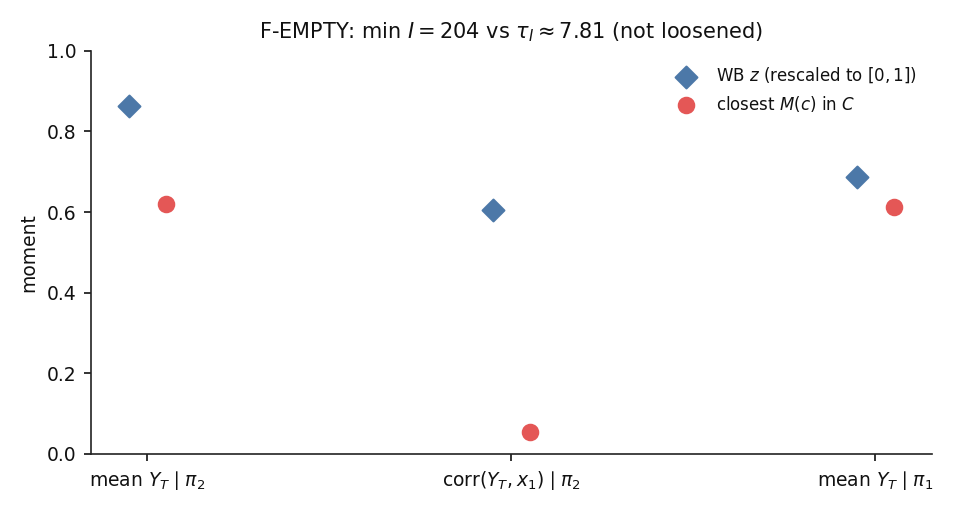
\includegraphics[width=0.82\linewidth]{fig-empty.png}
\end{center}
\captionof{figure}{F-EMPTY on World Bank $z$ (rescaled to $[0,1]$).
Closest simulated moments in $C$ versus anchors. Not a calibrated
world.}
\label{fig:empty}

\subsection{Planted $z$ left a fat NROY}
Against $z:=\widehat M(c^\star)$, three waves kept 202, then 416, then
373; union $|\NROY|=991$ (Figure~\ref{fig:waves}). The set did not
collapse. Closest survivor has $I\approx 0.002$. That is a close
score, not a recovery of $c^\star$: several coordinates, $\beta$ and
$\gamma$ among them, are not the plant values. That point is
$c_0^{\min I}$ by the pre-declared rule, not because it won on
$\theta$. Median-$I$ $c_0$ has $I\approx 2.02$ and a much larger
$\kappa$.

\begin{center}
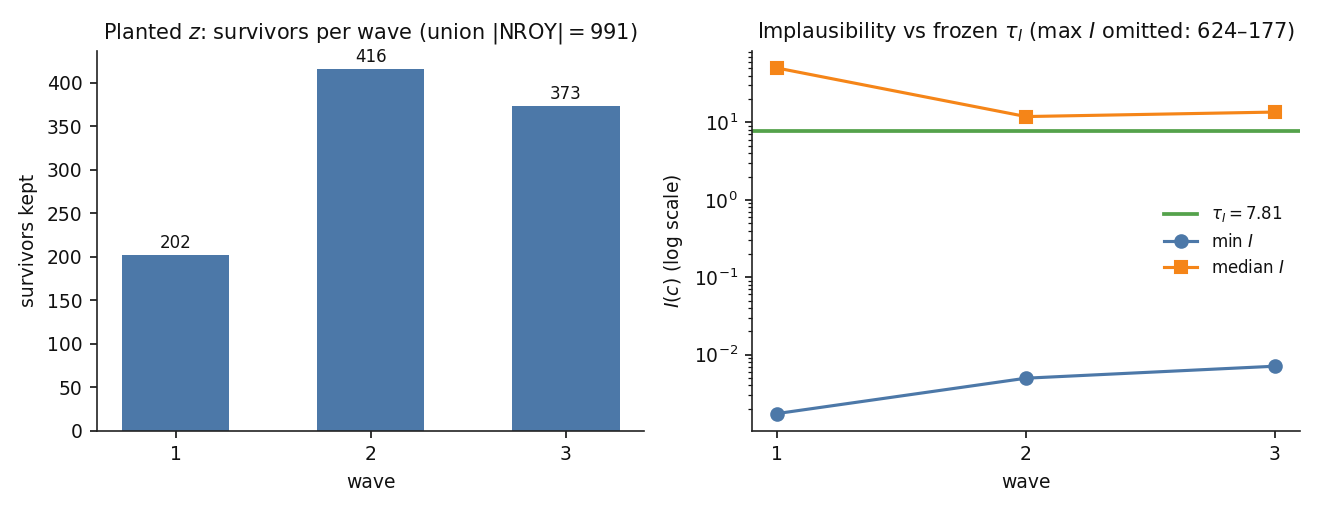
\includegraphics[width=\linewidth]{fig-waves.png}
\end{center}
\captionof{figure}{Planted history matching. Left: survivors per wave.
Right: min and median $I(c)$ against frozen $\thr$ (log scale). Later
waves concentrate; $\thr$ is not moved.}
\label{fig:waves}

\subsection{The image of $\theta_2$ is not a point}
At $c^\star$, hub vs none is $\theta_2=0.038$ (3.8~pp). Random vs none
is $\theta_1=0.036$. Targeting premium $\prem\approx 0.002$. In this
DGP, picking influencers barely beats picking at random. That is a
fact about this $c^\star$, not a theorem about targeting.

Among 400 sampled survivors, $\theta_2$ runs from 0.6~pp to 7.3~pp.
The planted 3.8 sits inside. Honest report:
$\Theta_{\hm}=[0.006,\,0.073]$, not $0.038$. Not a sampling
distribution and not a posterior.

Spillover $\delta_{\mathrm{spill}}(c^\star)\approx 0.008$; image
$\Theta_{\expset}\approx[-0.001,\,0.027]$. Direct-effect analogue
(hubs vs non-hubs \emph{inside} the random campaign)
$\delta_{\mathrm{dir}}(c^\star)\approx 0.34$.

\begin{center}
\small
\begin{tabular}{@{}lcc@{}}
\toprule
object & min $I$ world & median $I$ world \\
\midrule
$I(c_0)$ & $0.002$ & $2.02$ \\
$\theta_2(c_0)$ & $0.037$ & $0.063$ \\
OLS-HC1 $\Iols$ (hub panel) & $[0.326,\,0.346]$ & $[0.583,\,0.595]$ \\
$\Iols$ vs $\Theta_{\hm}$
  & $\Iols\cap\Theta_{\hm}=\emptyset$
  & $\Iols\cap\Theta_{\hm}=\emptyset$ \\
$\delta_{\mathrm{spill}}(c_0)$ & $0.006$ & $0.008$ \\
H\'ajek $\Ie$ & $[0.003,\,0.009]$ & $[0.006,\,0.011]$ \\
$\Ie$ vs $\Theta_{\expset}$
  & $\Ie\subset\interior(\Theta_{\expset})$
  & $\Ie\subset\interior(\Theta_{\expset})$ \\
oracle gate
  & $\delta_{\mathrm{spill}}(c_0)\in\Ie$
  & $\delta_{\mathrm{spill}}(c_0)\in\Ie$ \\
$\Theta_{\cv}$ & $[0.030,\,0.037]$ & $[0.056,\,0.063]$ \\
admitted $m$ & $m_1,m_2$ & $m_1,m_2$ \\
\bottomrule
\end{tabular}
\end{center}

\subsection{Overlay}
Figure~\ref{fig:overlay} is the money plot (two $c_0$, two functionals).
Figure~\ref{fig:intervals} repeats the same numbers on a shared axis so
the functional mismatch is visible without faceting.

At both $c_0$,
$\delta_{\mathrm{spill}}(c_0)\in\Ie$
(oracle gate: harness not broken) and
$\Ie\subset\interior(\Theta_{\expset})$.
Architecture handled; residual is which surviving $c$.
The sticker F-OVERCONF-E2 is that second inclusion.

OLS-HC1 on the hub panel lives near $0.33$--$0.59$, the neighbourhood
of $\delta_{\mathrm{dir}}$, not of $\theta_2$. $D$ \emph{is} ``being a
hub.'' The geometry is
$\Iols\cap\Theta_{\hm}=\emptyset$,
which is unnamed (neither $\Theta_{\hm}\subseteq\Iols$ nor
$\Iols\subset\interior(\Theta_{\hm})$).
Not ``OLS failed under interference.''

Oracle and noisy-survey scorings of $Y$ are admitted; the item that
loads on baseline propensity is excluded, as designed. $\Theta_{\cv}$
is a small scoring gap at a world, not a second NROY.

\begin{center}
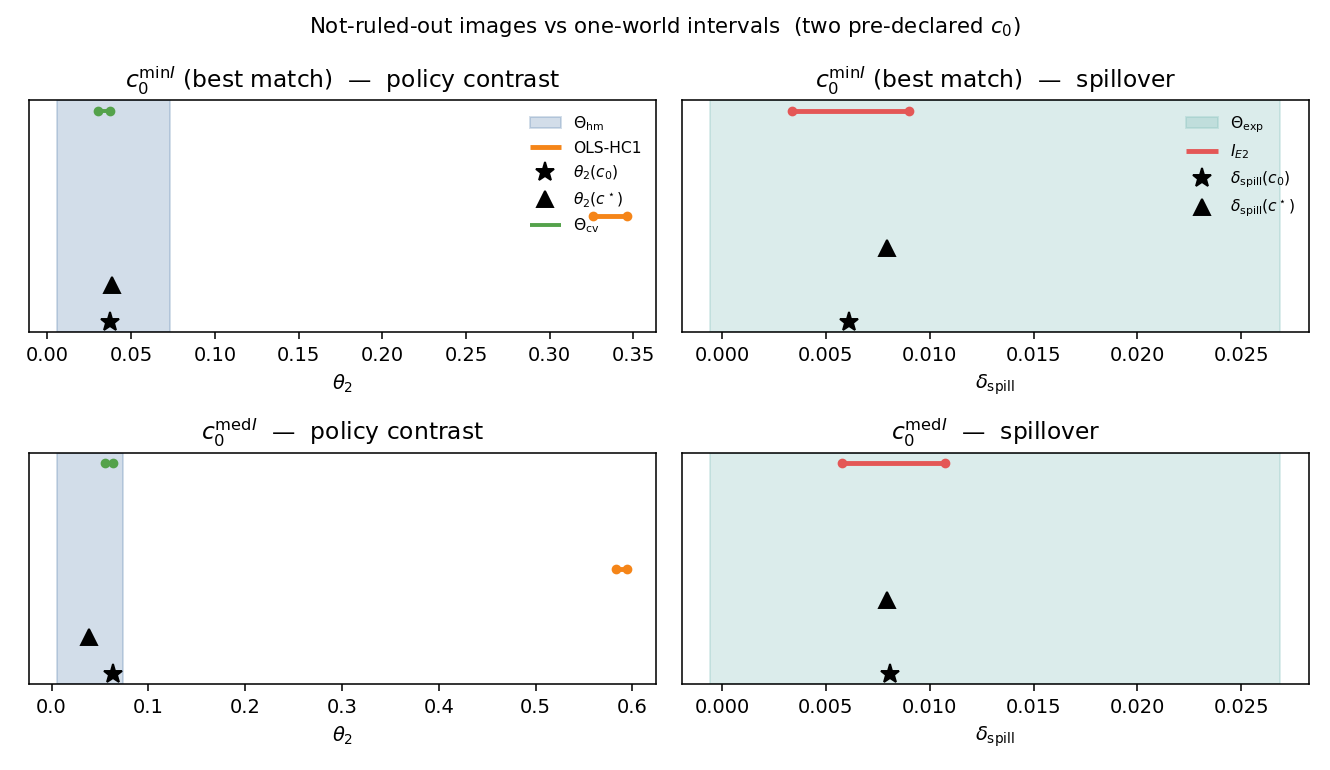
\includegraphics[width=\linewidth]{overlay.png}
\end{center}
\captionof{figure}{Not-ruled-out images versus one-world intervals at
two pre-declared $c_0$. Left: $\theta_2$ against $\Theta_{\hm}$; orange
is OLS-HC1 (not a forest). Right: $\delta_{\mathrm{spill}}$ against
$\Theta_{\expset}$; red is H\'ajek. Each interval against \emph{its own}
image.}
\label{fig:overlay}

\begin{center}
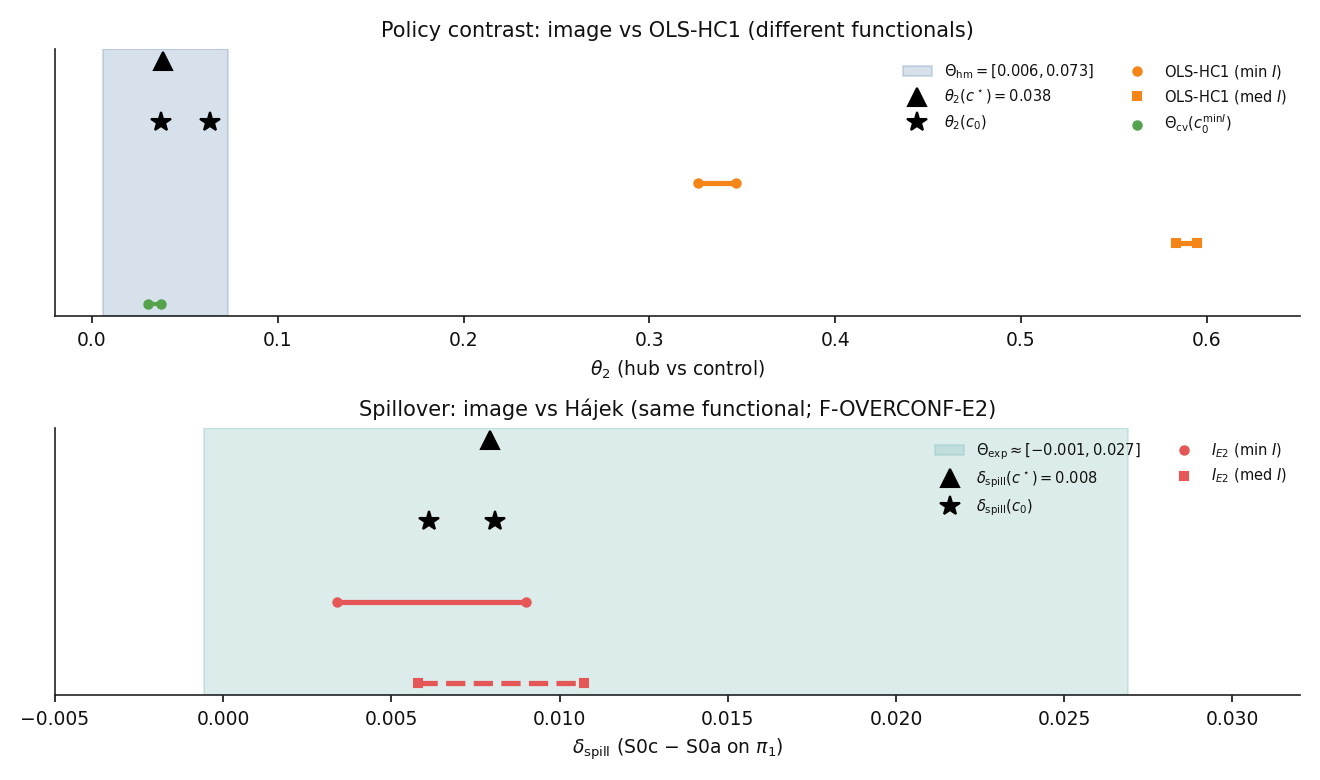
\includegraphics[width=\linewidth]{fig-intervals.png}
\end{center}
\captionof{figure}{Same objects on one axis per functional. Top:
$\Iols\cap\Theta_{\hm}=\emptyset$ because OLS is not $\theta_2$.
Bottom: $\delta_{\mathrm{spill}}(c_0)\in\Ie$ and
$\Ie\subset\interior(\Theta_{\expset})$.}
\label{fig:intervals}

%----------------------------------------------------------------
\section{Who should care --- and who should not}

Slogan-level novelty is weak. History matching already produces NROY
in input space (Craig, Goldstein, Vernon). Equifinality of ABMs is not
a discovery of this note (Beven; Williams--Guikema--Brown--Agrawal map
ensembles through policy). Partial identification already says: report
the set. Interference already has overall vs direct (Halloran,
Hudgens--Halloran). Honest forests and BCF already give intervals
\emph{given a panel}. None of those pieces is new. The remaining wedge,
if this is ever a paper, is the \emph{composition}: a named policy
contrast under interference, as the image of a history-matched set,
plus a measure-admission set, plus a paired SUTVA ruler and an
interference-aware estimator that isolates calibration as the residual,
on a simulator where truth is known. That is enough for an M.S.\
demonstration. It is not an Econometrica gap.

\paragraph{Anyone (method).}
Interesting if you already publish a policy number from a
\emph{calibrated simulator} (ABM, structural model, microsimulation)
and currently report Monte Carlo error at a staff $c_0$. The overlay
is a reporting split: sampling at a world is not uncertainty about
which worlds $z$ still allows. Empty NROY is a usable negative result
(the analog is rejected; do not loosen the cutoff). Width of $\Theta$
is measured, not assumed: here $\theta_2$ moves by about 7~pp across
survivors, not by ``anything.''

\paragraph{Causal inference, empirical.}
Not a new identifying strategy for the designs STP~517 actually
teaches. This procedure does not replace unconfoundedness, an
instrument, DiD, or an RDD. It does not estimate a CATE $\tau(x)$ on a
network. History matching does not identify heterogeneous treatment
effects.

It \emph{is} relevant to empirical CI in two narrower cases.

(1)~\emph{You are already using a model as the identification
vehicle} --- a structural DGP, an epidemic simulator, an ABM of a
campaign --- and then quoting one $\hat\theta$. Then the honest object
is the image of that $\theta$ over calibrations not ruled out by the
moments you were willing to match. One-world intervals (regression,
forests, BCF) remain honest \emph{at a world}. They are not the image.
If your paper is IV for wages, this is not your appendix.

(2)~\emph{Interference is in the DGP you wrote, and ITE is undefined.}
The well-posed object is a contrast of assignment rules. A SUTVA
learner on a targeting arm, where $D$ is a function of the graph,
identifies something in the neighbourhood of ``being a hub,'' not the
campaign contrast. That is an identification remark, not an estimator
bake-off. It is closer to STP~517 (name the estimand; when is
regression causal) than to ``run BCF on our panel.''

\paragraph{This PoC, specifically.}
The overlay is checkable because $z$ was \emph{planted}. The one
attempt at external $z$ (World Bank country totals) returned F-empty.
So this is not an empirical estimate of immunization policy, and it
should not be narrated as one. As a demonstration that the composition
can be run, with pre-registered verdicts including F-empty and
``neither F-*'', it is a completed lab. As a contribution to empirical
causal inference on real networks or real campaigns, it is not more
than that lab --- a toy with a clean object dictionary --- unless
someone later freezes a $z$ this kernel can actually speak to, without
moving $\thr$.

If the audience is ``applied micro who run regressions,'' treating this
as a portfolio piece that shows you can name functionals and not cheat
a cutoff is the honest pitch. If the audience already calibrates
simulators for policy, the overlay is the thing to steal; the village
story is not.

%----------------------------------------------------------------
\section{What the procedure is not}

\begin{itemize}
  \item Not a posterior over $c$, and not a distribution of treatment
        effects.
  \item Not a Manski identified set theorem-for-theorem. Same reporting
        logic; different incompleteness (calibration of a complete
        kernel, not missing counterfactuals); sampling and discrepancy
        already folded into $V$.
  \item Not a claim that equifinality of $\theta$ is guaranteed.
        Width is measured, not assumed.
  \item Not a finding that one-world estimators are bad at networks.
        They are honest for a world. The overlay asks whether one
        calibrated world is enough.
  \item Not a measurement model of the network. $A$ is frozen.
  \item Not an empirical immunization study. WB $z$ was rejected.
\end{itemize}

\vspace{1.2em}
{\small
\noindent\textit{Implementation.}
\texttt{ecn593-poc-abm}, AMENDMENT-02.
$|\NROY|=991$,
$\Theta_{\hm}=[0.006,0.073]$,
$\theta_2(c^\star)=0.038$.
Foil~1 estimator: OLS-HC1 (CausalForestDML did not import; not BCF).
Overlay: \texttt{figures/overlay.png}.
WB attempt archived as F-empty.
The declared exposure cut at $0.5$ is reported in the study packet
(\texttt{ecn593-applied-project}, section ``Declared cut at $0.5$''),
not here. This note does not repeat those digits. $\thr$ and $\delta$
were not moved for it.
Figures in this note are redrawn from the headline JSON; those waves
were not re-run.
}

\appendix
\section{Tamer (2010) and this image}
\label{sec:tamer}

This appendix is a written object map, not a new finding and not a
change to the freeze. It exists so a later thesis page, and an optional
four-minute extension after a seminar on Tamer, can use one text.
The seminar itself should teach Tamer's examples. Missing binary
outcomes and the \(2\times 2\) entry game are the right objects for an
audience meeting partial identification for the first time. The village
is a bad teaching example for his theorems: it is a different
incompleteness, and leading with it invites the collapse this note
already refuses.

\subsection{His objects}
Tamer's review treats identification as a menu, not a yes/no bit.
Assumptions plus the population distribution map to information about a
parameter. More assumptions buy a smaller set and less credibility; he
opens on Manski's law of decreasing credibility. The identified set is
the set of parameter values consistent with the maintained assumptions.
When that set is the argmin of an objective \(Q\), a sample analogue is
a level set \(\{y:Q_n(y)\le c_n\}\). He separates two targets
(his \S4.1): inference on the whole set, and inference on a true
parameter \(y^\star\) known only to lie in the set. Under
misspecification he notes there may be no true parameter in the set at
all --- only values that minimize a distance between the model class
and the distribution of the data (his footnote 14). His worked examples
are missing data (one of two potential outcomes is unobserved) and an
entry game (multiple equilibria). Neither is a calibrated simulator.

\subsection{Same reporting logic}
Do not replace a set by a convenient point. That sentence is the entire
overlap, and it is already the first paragraph of this note. The map
below uses only objects this note has already reported. It does not
import a new endpoint.

\begin{center}
\small
\begin{tabularx}{\linewidth}{@{}>{\raggedright\arraybackslash}p{0.30\linewidth}>{\raggedright\arraybackslash}X>{\raggedright\arraybackslash}X@{}}
\toprule
Tamer & This note & Stop \\
\midrule
Assumption menu
  & Frozen box \(C\), moments \(z\), discrepancy \(\delta\), cutoff \(\thr\), named \(\theta_2\)
  & Changing \(\thr\) after seeing the set is changing the menu. \\
Level set of an objective
  & \(\{c:I(c)\le\thr\}\). Planted run: \(|\NROY|=991\).
  & \(I\) is one joint ellipsoidal discrepancy, not a vector of moment inequalities. \(\thr\) is a pre-registered cutoff. It is not a \(c_n\to 0\) tuning sequence, and \(\NROY\) is not claimed to be a Hausdorff-consistent estimator of an identified set. \\
True parameter inside the set
  & Planted \(\theta_2(c^\star)=0.038\) sits in \(\Theta_{\hm}=[0.006,0.073]\). The report is the interval.
  & The interval is an image of a functional over a sample of survivors (\(S=400\)), not the identified set of \(c\), and not a posterior on worlds. \\
Misspecified distance set, no \(y^\star\) inside
  & World Bank \(z\): wave 1 kept 0 of 1000; minimum \(I=204\) against \(\thr\approx 7.81\).
  & Empty is a finding about the pair \((f,z)\). It is not a wide \(\Theta\), and it is not a warrant to loosen \(\thr\) or \(\delta\). \\
Stronger assumptions, tighter claim
  & OLS-HC1 at the two \(c_0\) is a few hundredths wide and disjoint from \(\Theta_{\hm}\).
  & That interval conditions on one world and on a SUTVA regression of hub status. Disjoint means a different functional, not ``the estimator failed.'' \\
\bottomrule
\end{tabularx}
\end{center}

The credible tightening in this design is not ``add a parametric
assumption and shrink \(\Theta_{\hm}\).'' It is to keep three
incompletenesses on separate axes, which the body of the note already
does: which \(c\) is not ruled out; which scoring of \(Y\) is admitted
at a world; which one-world interval is being quoted. Folding them into
one Manski box would buy a single picture by spending the distinction.

\subsection{Where the analogy stops}
\begin{itemize}
  \item Incompleteness here is which complete kernel still matches \(z\).
        Inside \(f\), both policies can be run. Missing \(Y_i(0)\) is
        Tamer's missing-data example. It is not this image.
  \item \(\Theta_{\hm}\) is a not-ruled-out \emph{image} of \(\theta_2\).
        Tamer's identified set is a set of parameter values. Stopping
        at \(\NROY\) would be stopping in his parameter space. The
        decision object is the image. Same reporting status; not his
        theorem.
  \item Membership in \(\NROY\) means not ruled out yet by \(I(c)\le\thr\).
        It does not mean observational equivalence, and it does not mean
        the point is known to be true.
  \item \(V\) already folds sampling variance and the discrepancy budget
        \(\delta\) into the score that rules \(c\) out. The computed
        image therefore mixes calibration uncertainty with those
        allowances. It is not a population identified set under exact
        moment equalities, and it is not a confidence set for one.
  \item Nothing in the results file is a Chernozhukov--Hong--Tamer
        region, a subsampled confidence set, or a uniformly valid
        interval for a partially identified parameter. Sampling
        uncertainty at one \(c_0\) is the foil interval. Width of
        \(\Theta_{\hm}\) is a different axis
        (Section~\ref{sec:geometry}).
\end{itemize}

\subsection{If the seminar gets four extra minutes}
Speak this, then stop. Do not show the overlay unless asked.

\begin{quote}
A simulator we wrote is a different incompleteness. Both policies can
be run, so the missing counterfactual in the missing-data example is
not what is unidentified. What the moments do not pin is the
calibration. The level set of the implausibility score is a set of
worlds. The object worth reporting is the image of a named policy
contrast over that set. In the planted run that image was about
7~percentage points wide, and a tight regression interval at one
surviving world missed it because the regression was not that
contrast. Same discipline as the review: do not replace the set by a
convenient point. Not the same theorem.
\end{quote}

Do not say that \(\Theta_{\hm}\) is a Manski identified set, that
\(\NROY\) points are observationally valid, that \(I(c)\) is a
moment-inequality model, or that the seminar has just seen Tamer's
inference section implemented. Those sentences are false of the
finished artifacts, and they are the ones a careful listener will ask
about.

\end{document}
